\clearpage

\section*{Problem Statement}
The link prediction (LP) problem is to predict future relationships from a given snapshot of a social network. E.g., one may wish to predict that a user will like a movie or book, or that two researchers will coauthor a paper, a user will endorse another on LinkedIn, or two users will become “friends” on Facebook. Apart from the obvious recommendation motive, LP can be useful in social search, such as Facebook Graph Search, as well as ranking goods or services based on not only real friends’ recommendations but also that of imputed social links.

\section*{Popular approaches}
Jaccard : The Jaccard index, also known as the Jaccard similarity coefficient (originally coined coefficient de communauté by Paul Jaccard), is a statistic used for comparing the similarity and diversity of sample sets. The Jaccard coefficient measures similarity between finite sample sets, and is defined as the size of the intersection divided by the size of the union of the sample sets
\begin{equation}
J(A,B) = \frac{\left\vert A \cap B \right\vert}{\left\vert A \cup B \right\vert}
\end{equation}
(If A and B are both empty, we define J(A,B) = 1.) Clearly,
$0 \leq J(A,B) \leq 1$
The MinHash min-wise independent permutations locality sensitive hashing scheme may be used to efficiently compute an accurate estimate of the Jaccard similarity coefficient of pairs of sets, where each set is represented by a constant-sized signature derived from the minimum values of a hash function.\\
The Jaccard distance, which measures dissimilarity between sample sets, is complementary to the Jaccard coefficient and is obtained by subtracting the Jaccard coefficient from 1, or, equivalently, by dividing the difference of the sizes of the union and the intersection of two sets by the size of the union:
Adamic Adar:To decide if nodes u and v may get linked, one strong signal is the number of common neighbors they already share. Adamic and Adar (AA) [1] refined this by a weighted counting: common neighbors who have many other neighbors are dialed down in importance:
\begin{equation}
SIM_{i,j}^{AA} = \sum_{k \in \Gamma(i) \cap \Gamma(j)} \frac{1}{\log {d(k)}}
\end{equation}
where d(k) is the degree of common neighbor k. The AA and RA predictors both penalize the contribution of high-degree common neighbors.


\section*{Our approach}
Unlike AA and other node-pair signals, our new approach recognizes that propensity of linkage is not purely a function of node similarity; it changes with neighborhood. Also, the presence or absence of edge (u, v) rarely determined by nodes far from u and v. So use a edge and triangulated dissimilarity based approach.


\section*{Defining edge dissimilarity}
Let $\Gamma(u)$ be the (immediate) neighbors of u. We will model the edge dissimilarity between u and v as
\begin{equation}
\Delta_{w}(u,v) = w_{uv} . |\Theta_u - \Theta_v|
\end{equation}
 $w_{uv}$ is the weight vector fitted locally for u, v. 
 
\section*{Triangulated Dissimilarity}
The optimization program outputs $w_{uv}^{\ast}$, from which we can compute 
\begin{equation}
\delta_{uv} = w_{uv}^{\ast} . |\Theta_u - \Theta_v|
\end{equation}
Using only this may not be useful for learning a global consistent model. Therefore, we also compute the triangulated dissimilarity
\begin{equation}
\Delta_{w_{xy}}^{x,y} = \sum_{x \in Q,y \in Graph} \frac{\sum_{i \in T(x) \cap T(y)} \Delta_{w_{xy}}(i,x) + \Delta_{w_{xy}}(i,y)}{ |T(x) \cap T(y)|}
\end{equation}
Finally we use this as the score metric,
\begin{equation}
f(u,v)[LL] = \Delta_{w^{*}}(u,v) - \delta_{u,v}
\end{equation}

\section*{Objective function selection}
We assume that the value of the dissimilarity function is low for node pairs which have an edge connecting them and relatively higher for node pairs which are not neighbours. Under these impositions, we wish to minimize the sum of the dissimilarity values of x and y with their common neighbours. This is because this minimization would in turn give the maximum possibility of an edge between x and y that may appear in future. So our objective is to find optimal w, so that the triangulated dissimilarity
\begin{equation}
\Delta^{x,y} = min_{w} \Delta_{w}^{xy}
\end{equation}
is minimized.
\\
Apart from that we want to chose the w vectors in such a manner that $\delta_{uv}$ is larger than nodes which are known to be connected and also smaller than the nodes. So in both cases we can form our constraints in the following manner
\begin{equation}
\sum_{i \in \Gamma(x) \setminus \Gamma(y)} \Delta_{w} (i,x) \leq \alpha \Delta_{w}^{xy}
\end{equation}
\begin{equation}
\sum_{i \in \Gamma(y) \setminus \Gamma(x)} \Delta_{w} (i,y) \leq \alpha \Delta_{w}^{xy}
\end{equation}
\begin{equation}
\sum_{i \in \Gamma(y) \setminus \Gamma(x)} \Delta_{w} (i,x) \geq \alpha \Delta_{w}^{xy}
\end{equation}
\begin{equation}
\sum_{i \in \Gamma(x) \setminus \Gamma(y)} \Delta_{w} (i,y) \geq \alpha \Delta_{w}^{xy}
\end{equation}
So to find the $w$ for the $\delta_{uv}$ computation we can use the constraints as constraints of an SVM. Because as we are trying to minimize the $|w|^2$ which is a classic QP optimization wrt some linear constraints but as our equations can be approximated as SVM constraints (i.e. approximating $ \leq 0$ as $\leq -1$ and $\geq 0$ as $\geq 1$). So for each query-node pair we can run an SVM and find the required $w$ vector.
\\
Similarly minimizing the triangulated dissimilarity is exactly a classic LP problem wrt to the given constraints. We can then simply compute the actual triangulated dissimilarity for the query-node pair and compute the final score.


\section*{Integrated Single Stage Learning}
In both LP and QP based approach though we are using the help of the neighborhood, but in every query-node computation, when we are going to compute both edge and reference dissimilarity we are using their own weight vector i.e. for different query-node pair even in computing the same dissimilarity. One way to encounter this is to use an integrated one step learning approach. Instead of learning for a specific query-node pair we try to learn all query-node pair together. But the main drawback in this approach is problem with scaling. If the graph is in the order of thousands of nodes then depending the query size and feature vector size the QP and LP problems can be in the size (number of variables) of millions. So solving them is not a very practical idea indeed. So we are trying to keep both the essence. Instead of learning the whole graph together we can use a per query based learning or may also define a threshold on number of variables. Whenever the quota is filled we solve the LP and QP problems and then go on solving the rest. Though this decouples the theoretical QP and LP problems still we can do some experimentation.



\section*{LP Based approach}
We used the original constraints on a LP solver (GLPK - GNU Linear Programming toolKit - Simplex algorithm). we ran our implementation on the movielens (3952 nodes) data set and our MAP was .53 (which is still not better than the two step learning approach). Here we also used the same weight values for triangulated and edge dissimilarity value computation.

   
\section*{Adding more features}
After the previous work instead of going to the hybrid approaches as suggested earlier we tried to introduce new featur - Hitting time, Commute Time, Katz Score, Preferential Attachment, Jaccard Score, Adamic Adar, Common Neighbor score and GraphDistance \cite{linkpredsocial}. Here we give a brief overview of the features. After that we have done a quadratic coupling study of features.
% hitting time and commute time
\\
A random walk on $G$ starts at a node $x$ and iteratively moves to a neighbor of $x$ chosen uniformly at random from the set $\Gamma(x)$ (set of direct neighbors of the node $x$). The hitting time $H_{x,y}$ from $x$ to $y$ is the expected number of steps required for a random walk starting at $x$ to reach $y$.Because the hitting time is not in general symmetric, it is also natural to consider the commute time $C_{x,y} := H_{x,y} + H_{y,x}$. From \cite{hittingtime} we find that we can easily compute hitting time matrix $H$ according to the following formula $H = 1 \dot{}  [diag( \widetilde{Z})]^{T} - \widetilde{Z}$ where $\widetilde{Z}$ is the scaled fundamental matrix as defined in \cite{hittingtime}.
\\
%Katz Score
In this work we have also incorporated two new features - Preferential Attachment and Katz Score. Katz Score is among the methods to refine the notion of shortest paths by considering the set of all paths between two nodes. Katz defines a measure that directly sums over this collection of paths, exponentially damped by length to count short paths more heavily. This notion leads to the measure $Score(x,y) := \sum\limits_{l=1}^{\infty} \beta^l |paths_{x,y}^{<l>}|$ where $paths_{x,y}$ is the set of all length- paths from $x$ to $y$, and $\beta > 0$ is a parameter of the predictor (A very small $\beta$ yields predictions much like common neighbors, because paths of length three or more contribute very little to the summation). We can easily find a closed expression of the $Score$ matrix. By definion the $score = \sum\limits_{l=1}^{\infty} \beta^l M^l$ (where M is the adjacency matrix of the graph). Now $Score + I = \sum\limits_{l=0}^{\infty} \beta^l M^l = (I-\beta M)^{-1} \iff Score = (I-\beta M)^{-1} - I$ From the definition of Katz score, as we are considering all possible paths it also captures the notion of the global structure of the Graph.
\\
%Preferentail Attachment Score
Our framework also tries to capture the the local effects by introducing the Preferential Attachment feature. For a node $x$, let $\Gamma (x)$ denote the set of neighbors of $x$. Now the definition of Preferential Attachment comes from the growth model. We know if we introduce a new node then $x$ will be one of its neighbors with probability $|\Gamma(x)|$. Now in our graphs are not temporal and as both $x$ and $y$ already exists so to capture their local similarity be good approach would be to define $PA(x,y) := |\Gamma(x)|.|\Gamma(y)|$.
\\
% common neighbor and graph distance
The common neighbor score is defined as $score(x, y) := |\Gamma(x) \cap \Gamma(y)|$, the number of neighbors that $x$ and $y$ have in common. And graph distance is basically the all pair shortest path distance which we computed using Floyd Warshall Algorithm. For all these methods we have written MATLAB scripts.

\section*{Survey of Matrix Factorization in Link Prediction}
We studied matrix factorization techniques for Link Prediction Problems. Till now we have computed features for nodes and node-node pairs. Also using the adjacency information with various techniques we have also learned the pair wise similarity vectors among all pairs. So basically in a we can write the overall link score in a generic manner like this
\begin{equation}
	G(i,j) = min_{\theta} L (f_{D}(z_{ij};w) + f_{M}(x_i,x_j,;v))
\end{equation}
Here $w$ and $v$ are weight vectors that we learn from the train data by minimizing some loss function (with some proper regularizer to stop the parameters from blow up).  On the contray in the matrix factorization based Latent Feature model we try to factorize the graph $G = L ( U A U^{T})$. Where $L$ is a linking function applied on each of elements of the matrix. So the optimization problem can be formally posed as
\begin{equation}
	G(i,j,U,A) =  L (u_{i}^{T} A u_{j})
\end{equation}
Now as we have a linking function we can now use it for minimizing a loss function with a suitable regularizer. So this structural node, node-node scores and latent scores can be combined as a single optimization problem in the following manner,
\begin{multline}
	U,A,w,v,b = argmin_{U,A,w,v,b} \frac{1}{|O|}  \sum_{(i,j)}\in O  Loss( G(i,j), \\
	 L(u_i^T A u_j + b_i + b_j + f_D(z_{ij};w) + f_M(x_i,x_j;v))) + \Omega(U,A,w,v,b)
\end{multline}
Where $\Omega$ is a provided regularizer, and $Loss$ and $l$ are a given loss and regularization function. For example we can use square or logarithmic loss and sigmoid linking function. Also we can try to learn $f_D(z_{ij};w) = w^T z_{ij}$ and $f_M(x_i,x_j;v) = v^T x_i + v^T x_j$. However to learn non linear features in a better manner we can define the  $f_M(x_i,x_j;v) =  x_i^T v x_j$ where  V is a $d \times d$ matrix where $d$ is the linear node feature dimension. Now $v$ can be symmetric matrix if the given graph is symmetric. We can also approximate $v$ as $D + A^TB$ where $D$ is a diagonal matrix. So its obvious that we can plug our known scores in the top level optimizer problem. However this suffers from the issue of clas imbalance which is predominant in Link Prediction Datasets. So to ovrcome this we directly optimize to maximize the AUC of the ROC.  To do this, we begin with the pairwise SVMRank framework .
Consider a binary classification scenario with training set $\lbrace (x_i, y_i) \rbrace$, and let$P = \lbrace i : y_i = 1 \rbrace $ and
$N = \lbrace i : y_i = 0 \rbrace $. The empirical AUC of a linear classifier with weight $w$ is
\begin{equation}
A = \frac{1}{|N||P|} \sum_{i \in P} \sum_{j \in N} 1 [w^T x_i > w^T x_J]
\end{equation}
So the problem of optimizing $w$ can be written as 
\begin{equation}
w = argmin_w \frac{1}{|N||P|} \sum_{i \in P} \sum_{j \in N} 1 [w^T (x_i - x_J) < 0]
\end{equation}
We can add a suitable regularizer so that $w$ does not overfit. So in our specific case we can reformulate the top level optimization problem as
\begin{multline}
U,A,v,w,b = argmin_{U,A,v,w,b} \frac{1}{|O|} \sum\limits_{i=1}^n \sum\limits_{j \in O^{+} k \in O^{-}} Loss( \\
 L(u_i^T A (u_j - u_k) + b_i + b_j + f_D(z_{ij};w) + f_M(x_i,x_j;v)), 1) + \Omega(U,A,w,v,b)
\end{multline}
Now we could have used gradient descent to optimize this but for a function of $Q(w) = \sum\limits_{i = 1}^n Q_i(w)$, the update step is $w_n = w_{n-1}  - \bigtriangledown Q(w_{n-1}) = w_{n-1} - \sum\limits_{i = 1}^n  \bigtriangledown Q_i(w_{n-1})$. As in our case we have a quadratic number of terms in the optimization function it will be difficult fot standard gradient descent. So we used Stochastic Gradient Descent. In stochastic gradient descent.  We randomly shuffle the indexes of the sumation functions and we do gradient descent for that function only ie. $w_n = w_{n-1}  - \bigtriangledown Q(w_{n-1})$ and in each epoch each of the sumation is taken exacly once but in a random order. We repeat the epochs until some provided convergence condition is met. So in our specific case we will select a $i$ and $j$ in each step and find the optimal parameters.

\section*{Experimental results}
Now for this specific study we have used our Movielens, Netflix, Cora, Cite, WebKb, Conflict and Prot-Prot datasets to do the experiments. We used SGD based matrix factorization to find optimum model parameters in each case. 
%In Figure~\ref{fig:arbitration_study} we show the linear feature selection study. Here on average we find that if we take the 

%\begin{figure}
%\centering
%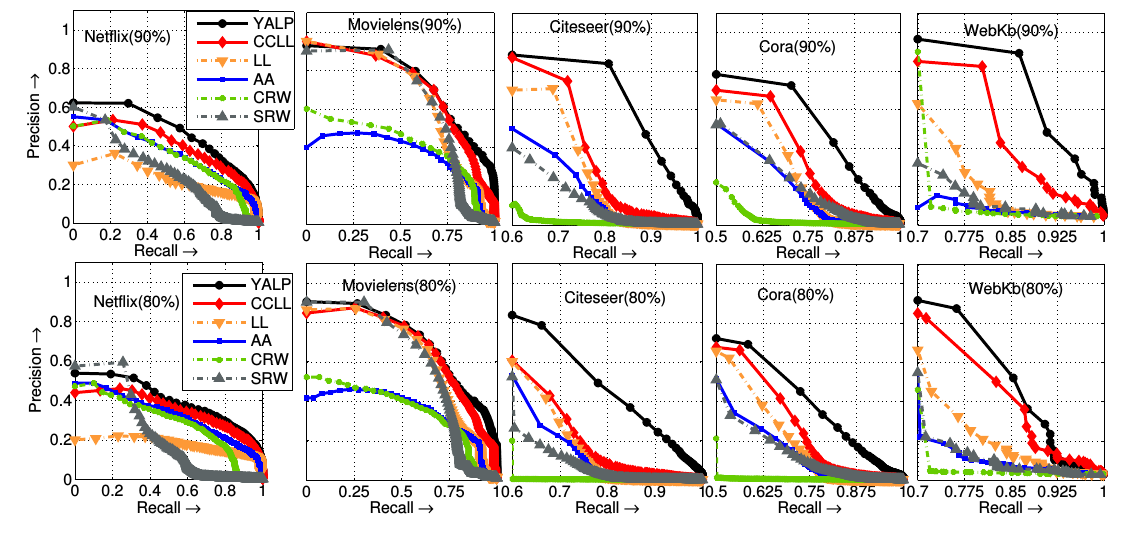
\includegraphics[width=\textwidth,height=\textheight,keepaspectratio]{link_prediction/images/precision_recall.png}
%\caption{Precision vs. recall curves for all data sets and algorithms}
%\label{fig:precion_recall}
%\end{figure}


\section*{Tools Used}
C++, GLPK, Boost Graph Library, Matlab, Python
